\documentclass[a4paper,12pt]{report}
\usepackage{CJKutf8}
\usepackage{graphicx}
\usepackage{float}
\usepackage{subfigure}
\usepackage[colorlinks = true,linkcolor = black, urlcolor  = blue,]{hyperref}
\title{建模報告}
\author{鄭詠澤\and 陳郁錡\and 游家竣\and 梁恩齊}
\date{\today}

\begin{document}
\begin{CJK*}{UTF8}{bkai}
\maketitle
\tableofcontents
\chapter{題目解析}

\section{題目敘述}

題目解釋說我們需要設計一個 $V(\rho)$ 當速度函數,然後給定不同條件看有沒有塞車現象。\\

因此我們知道密度跟速度是有關係的,而速度這個函數本身跟位置還有時間是有關係的,所以我們要判斷的關係是車流密度究竟與 $X_t$ 有什麼關係,有了這個關係後我們就可以用速度的上下限去看塞車的現象。\\

車流量的定義是單位時間內上去的車子的量,因為跟距離有關係,如果我們固定某個車速,給定某一段 L,那我們就可以知道在某個車速的情況下,每過一段時間有多少車上來。 

\chapter{解題想法}

\section{道路構思}

由於在思考時我們希望一台車一下去就會有另外一台車上道路,如此一來密度才不會改變,因此我們把車道想成這樣:

\begin{figure}[H] 
\centering 
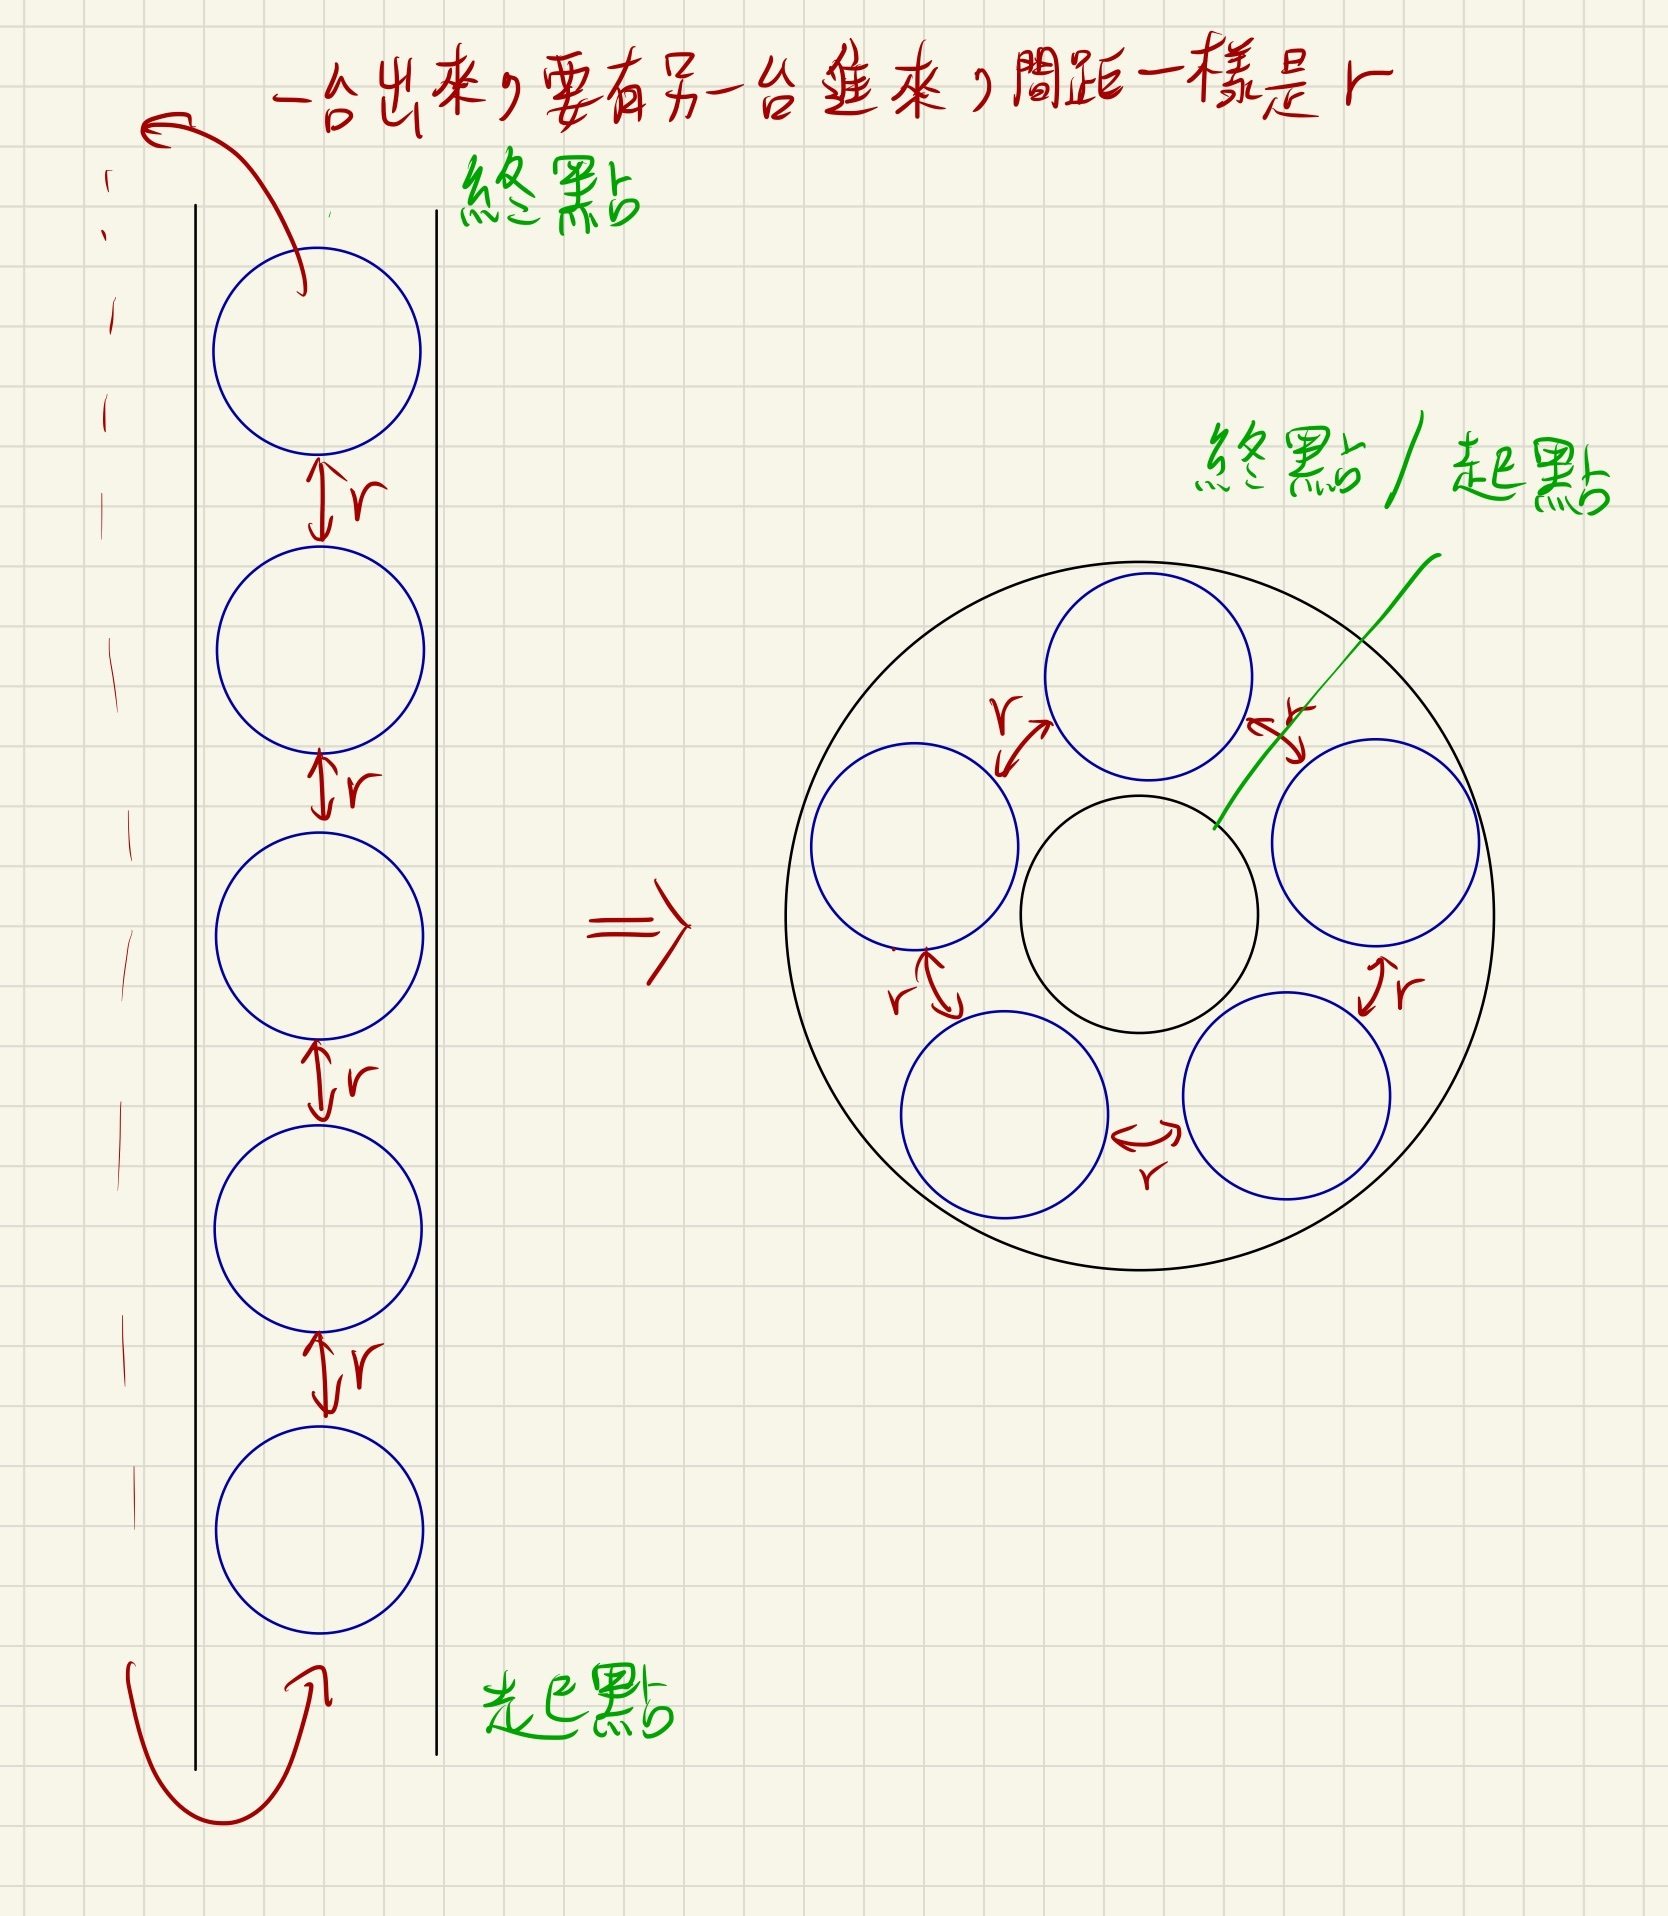
\includegraphics[width=0.6\textwidth]{11-2} 
\caption{車道構思圖} 
\label{Fig.main2} 
\end{figure}

這樣就好像一台車一下道路時馬上便有另一台車上道路,符合我們的需求。 \newpage

\section{速度問題}

而速度 A、B、C 的關係圖會如下所示:

\begin{figure}[H] 
\centering 
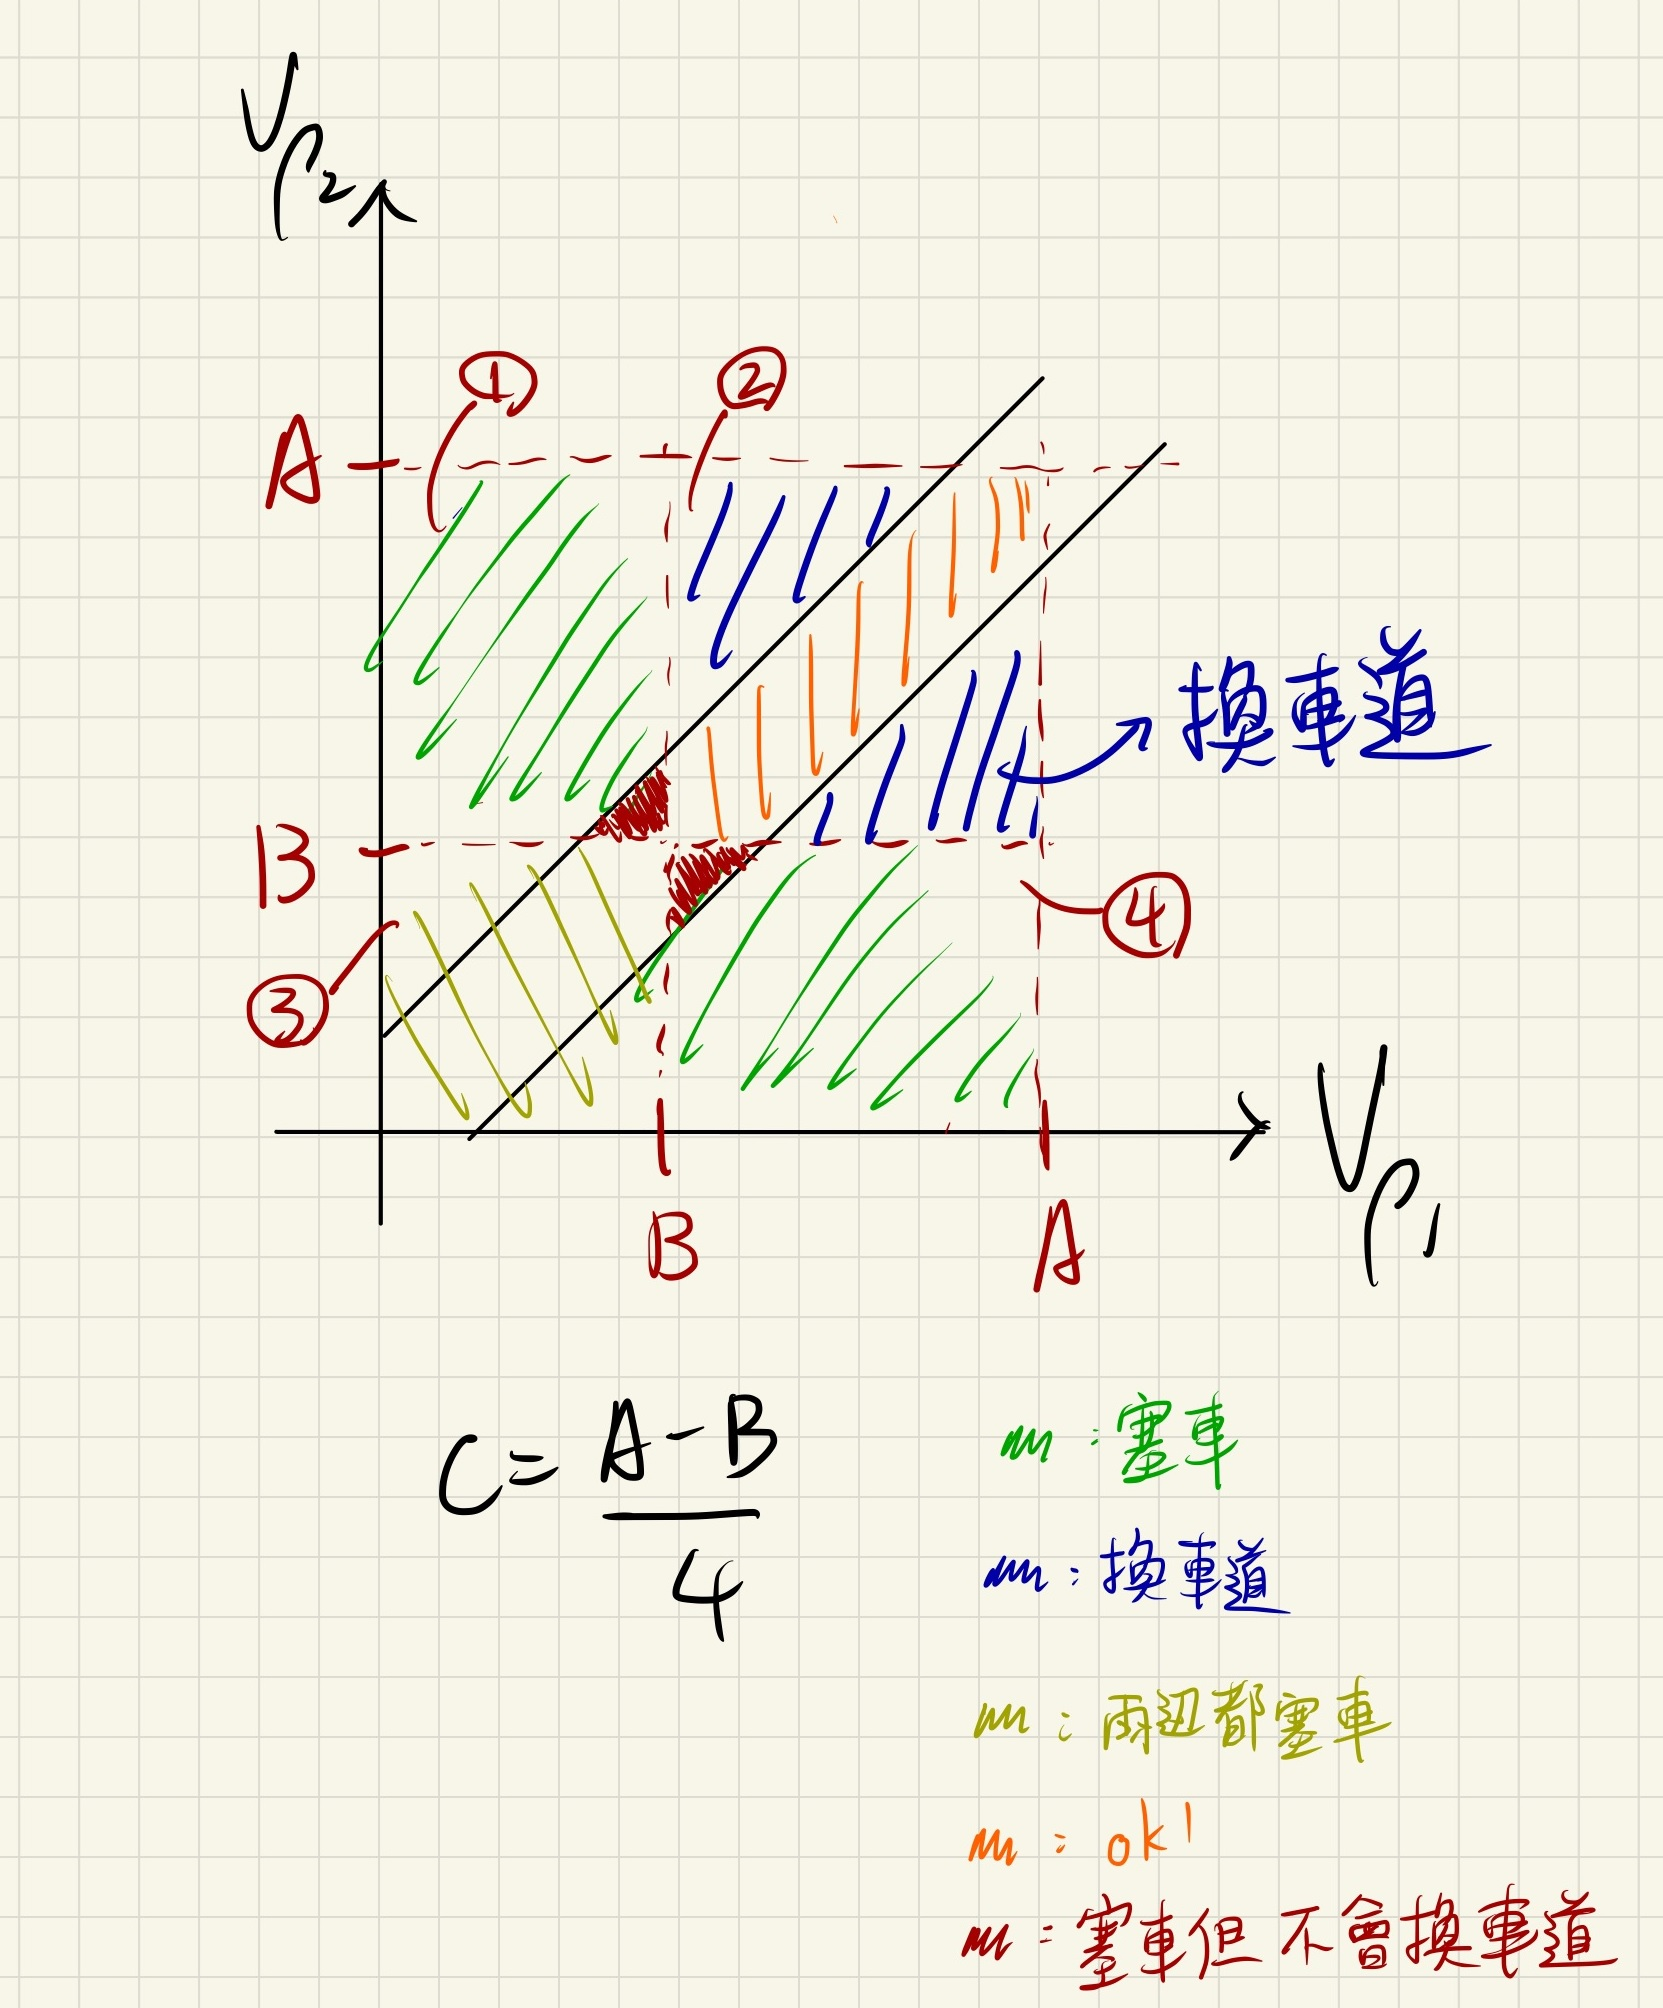
\includegraphics[width=0.7\textwidth]{11-1} 
\caption{車輛速度關係圖} 
\label{Fig.main2} 
\end{figure}

A、B、C 都會變動,變動的方式是上圖的 A、B 於軸上移動, C 如果越大,三角形會越小(那兩條線會往外面擠)\\

畫藍色斜線部分是沒有塞車且合理的車速情況下,相差大於 C 的,所以要做車道轉換\\

而我們以某種方式去迭代時,轉換後一定會有一組新的 $V_1$、$V_2$,所以狀態一定會變,而我們要做的事就是看迭代後該點是不是仍在斜線裡面,現在這是一個連續動作,車道轉換會導致塞車的情況,在迭代過程中,如果跑出這個矩形,就是塞車。另外速度 $B$ 是塞車的臨界點,也就是產生最大流量的時候,

\section{資料問題}

資料部份我們會到交通部的交通資料庫下載,下載下來會是個 XML 檔,資料的格式有一份\href{https://www.motc.gov.tw/uploaddowndoc?file=bussiness/201810051359110.pdf&filedisplay=%E9%99%84%E4%BB%B62-%E4%BA%A4%E9%80%9A%E9%83%A8%E5%8D%B3%E6%99%82%E8%B7%AF%E6%B3%81%E8%B3%87%E6%96%99%E6%A8%99%E6%BA%96v2-XML%E6%A8%99%E6%BA%96%E6%A0%BC%E5%BC%8F%E6%96%87%E4%BB%B6-20180802.pdf&flag=doc}{文件}內有解釋,我們可以透過這些資料來檢查找出來的 $V(\rho)$ 是不是合理的。

\section{找\ $V({\rho})$ 函數}

找關係有很多種方法,像是多項式的擬合,或是有一些經驗方程可以用,我們有找到一份\href{https://www.ceci.org.tw/Upload/Download/8B04AEBF-C160-477C-B6E3-63FA9A3BA096.pdf}{文件},裡面寫了許多模型,像是 Greenshield、Greenberg、Underwood 等等。\\

我們知道流量 = 速度 $\times$ 密度,理論上如果固定速度,當密度上升時,流量也會跟著上升。然而現實生活中不可能如此,因為密度是有限制的,當密度大到某個程度時,速度便會下降,這兩個不是完全獨立的變數。\\

所以圖形畫出來不會是條斜直線,而會是個曲線,wiki 上有個圖形長這樣:

\begin{figure}[H] 
\centering 
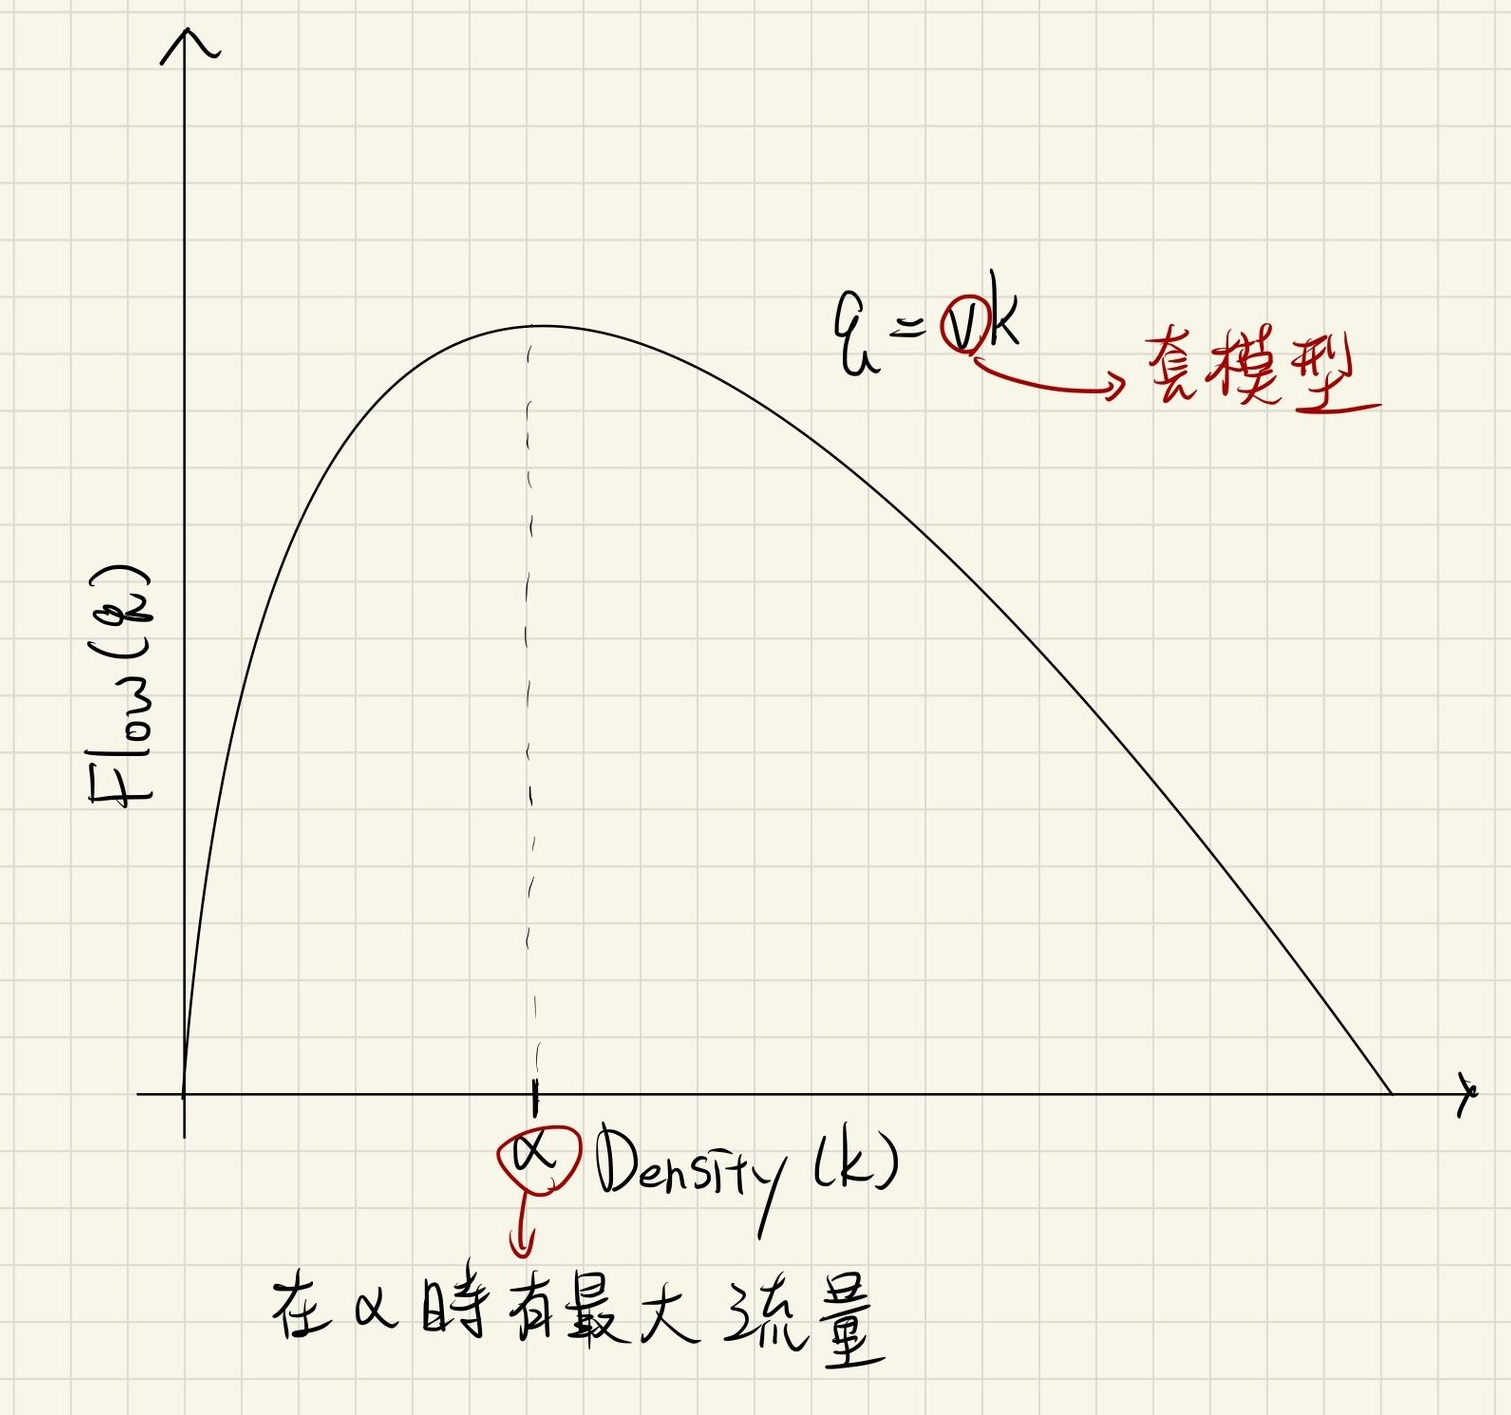
\includegraphics[width=0.5\textwidth]{11-3} 
\caption{密度與流量關係圖}
\label{Fig.main2} 
\end{figure}

上圖是流體模型的基本圖,可以看見圖形是個拋物線,如果我們有速度與密度的關係,就可以畫出類似的圖,上圖在某個密度 $\alpha$ 時會有最大流量,如果密度再繼續上升,流量便會下降,可以想像成開始慢慢在塞車了。

\section{換車道}

如果我們知道車速,便會知道密度是多少,如此一來就可以看見兩邊的密度高低與密度差,因此現在問題就是車子要不要轉換車道,於什麼樣的密度下要轉換車道,不是一到那個密度就會換,而是到了多久後才會轉換。\\

而換車道也需要一個模型,每次可能是幾台或是一個比例的車去轉換,也就是說這件事其實是一個離散的問題,車子不會轉到中間停下來,一定會整台車過去。\\

因此我們想建立兩個車道,這兩個車道要有一些關係,兩個車道設計可能是一樣的,然後中間有個高架橋之類的,這樣一來那個車道的速度就會取決於那個車道上的密度。\\

我們認為在巨觀下會發生動態平衡,也就是過去的車輛與回來的車輛是差不多的。

\section{目前的困難}

\begin{itemize}
\item[1.] 車子資料解讀有問題,我們不知道某個車道最大的 Q 是要怎麼找,也許是我們要自己設?\\

\item[2.] 速度其實也不太清楚,在區段上面的速度的平均值我們不太知道其意義為何。
\end{itemize}

\end{CJK*}
\end{document}